\documentclass{ximera}

%\usepackage{todonotes}

\newcommand{\todo}{}

\usepackage{esint} % for \oiint
\ifxake%%https://math.meta.stackexchange.com/questions/9973/how-do-you-render-a-closed-surface-double-integral
\renewcommand{\oiint}{{\large\bigcirc}\kern-1.56em\iint}
\fi


\graphicspath{
  {./}
  {ximeraTutorial/}
  {basicPhilosophy/}
  {functionsOfSeveralVariables/}
  {normalVectors/}
  {lagrangeMultipliers/}
  {vectorFields/}
  {greensTheorem/}
  {shapeOfThingsToCome/}
  {dotProducts/}
  {partialDerivativesAndTheGradientVector/}
  {../productAndQuotientRules/exercises/}
  {../normalVectors/exercisesParametricPlots/}
  {../continuityOfFunctionsOfSeveralVariables/exercises/}
  {../partialDerivativesAndTheGradientVector/exercises/}
  {../directionalDerivativeAndChainRule/exercises/}
  {../commonCoordinates/exercisesCylindricalCoordinates/}
  {../commonCoordinates/exercisesSphericalCoordinates/}
  {../greensTheorem/exercisesCurlAndLineIntegrals/}
  {../greensTheorem/exercisesDivergenceAndLineIntegrals/}
  {../shapeOfThingsToCome/exercisesDivergenceTheorem/}
  {../greensTheorem/}
  {../shapeOfThingsToCome/}
  {../separableDifferentialEquations/exercises/}
  {vectorFields/}
}

\newcommand{\mooculus}{\textsf{\textbf{MOOC}\textnormal{\textsf{ULUS}}}}

\usepackage{tkz-euclide}
\usepackage{tikz}
\usepackage{tikz-cd}
\usetikzlibrary{arrows}
\tikzset{>=stealth,commutative diagrams/.cd,
  arrow style=tikz,diagrams={>=stealth}} %% cool arrow head
\tikzset{shorten <>/.style={ shorten >=#1, shorten <=#1 } } %% allows shorter vectors

\usetikzlibrary{backgrounds} %% for boxes around graphs
\usetikzlibrary{shapes,positioning}  %% Clouds and stars
\usetikzlibrary{matrix} %% for matrix
\usepgfplotslibrary{polar} %% for polar plots
\usepgfplotslibrary{fillbetween} %% to shade area between curves in TikZ
%\usetkzobj{all}
\usepackage[makeroom]{cancel} %% for strike outs
%\usepackage{mathtools} %% for pretty underbrace % Breaks Ximera
%\usepackage{multicol}
\usepackage{pgffor} %% required for integral for loops



%% http://tex.stackexchange.com/questions/66490/drawing-a-tikz-arc-specifying-the-center
%% Draws beach ball
\tikzset{pics/carc/.style args={#1:#2:#3}{code={\draw[pic actions] (#1:#3) arc(#1:#2:#3);}}}



\usepackage{array}
\setlength{\extrarowheight}{+.1cm}
\newdimen\digitwidth
\settowidth\digitwidth{9}
\def\divrule#1#2{
\noalign{\moveright#1\digitwidth
\vbox{\hrule width#2\digitwidth}}}




% \newcommand{\RR}{\mathbb R}
% \newcommand{\R}{\mathbb R}
% \newcommand{\N}{\mathbb N}
% \newcommand{\Z}{\mathbb Z}

\newcommand{\sagemath}{\textsf{SageMath}}


%\renewcommand{\d}{\,d\!}
%\renewcommand{\d}{\mathop{}\!d}
%\newcommand{\dd}[2][]{\frac{\d #1}{\d #2}}
%\newcommand{\pp}[2][]{\frac{\partial #1}{\partial #2}}
% \renewcommand{\l}{\ell}
%\newcommand{\ddx}{\frac{d}{\d x}}

% \newcommand{\zeroOverZero}{\ensuremath{\boldsymbol{\tfrac{0}{0}}}}
%\newcommand{\inftyOverInfty}{\ensuremath{\boldsymbol{\tfrac{\infty}{\infty}}}}
%\newcommand{\zeroOverInfty}{\ensuremath{\boldsymbol{\tfrac{0}{\infty}}}}
%\newcommand{\zeroTimesInfty}{\ensuremath{\small\boldsymbol{0\cdot \infty}}}
%\newcommand{\inftyMinusInfty}{\ensuremath{\small\boldsymbol{\infty - \infty}}}
%\newcommand{\oneToInfty}{\ensuremath{\boldsymbol{1^\infty}}}
%\newcommand{\zeroToZero}{\ensuremath{\boldsymbol{0^0}}}
%\newcommand{\inftyToZero}{\ensuremath{\boldsymbol{\infty^0}}}



% \newcommand{\numOverZero}{\ensuremath{\boldsymbol{\tfrac{\#}{0}}}}
% \newcommand{\dfn}{\textbf}
% \newcommand{\unit}{\,\mathrm}
% \newcommand{\unit}{\mathop{}\!\mathrm}
% \newcommand{\eval}[1]{\bigg[ #1 \bigg]}
% \newcommand{\seq}[1]{\left( #1 \right)}
% \renewcommand{\epsilon}{\varepsilon}
% \renewcommand{\phi}{\varphi}


% \renewcommand{\iff}{\Leftrightarrow}

% \DeclareMathOperator{\arccot}{arccot}
% \DeclareMathOperator{\arcsec}{arcsec}
% \DeclareMathOperator{\arccsc}{arccsc}
% \DeclareMathOperator{\si}{Si}
% \DeclareMathOperator{\scal}{scal}
% \DeclareMathOperator{\sign}{sign}


%% \newcommand{\tightoverset}[2]{% for arrow vec
%%   \mathop{#2}\limits^{\vbox to -.5ex{\kern-0.75ex\hbox{$#1$}\vss}}}
% \newcommand{\arrowvec}[1]{{\overset{\rightharpoonup}{#1}}}
% \renewcommand{\vec}[1]{\arrowvec{\mathbf{#1}}}
% \renewcommand{\vec}[1]{{\overset{\boldsymbol{\rightharpoonup}}{\mathbf{#1}}}}

% \newcommand{\point}[1]{\left(#1\right)} %this allows \vector{ to be changed to \vector{ with a quick find and replace
% \newcommand{\pt}[1]{\mathbf{#1}} %this allows \vec{ to be changed to \vec{ with a quick find and replace
% \newcommand{\Lim}[2]{\lim_{\point{#1} \to \point{#2}}} %Bart, I changed this to point since I want to use it.  It runs through both of the exercise and exerciseE files in limits section, which is why it was in each document to start with.

% \DeclareMathOperator{\proj}{\mathbf{proj}}
% \newcommand{\veci}{{\boldsymbol{\hat{\imath}}}}
% \newcommand{\vecj}{{\boldsymbol{\hat{\jmath}}}}
% \newcommand{\veck}{{\boldsymbol{\hat{k}}}}
% \newcommand{\vecl}{\vec{\boldsymbol{\l}}}
% \newcommand{\uvec}[1]{\mathbf{\hat{#1}}}
% \newcommand{\utan}{\mathbf{\hat{t}}}
% \newcommand{\unormal}{\mathbf{\hat{n}}}
% \newcommand{\ubinormal}{\mathbf{\hat{b}}}

% \newcommand{\dotp}{\bullet}
% \newcommand{\cross}{\boldsymbol\times}
% \newcommand{\grad}{\boldsymbol\nabla}
% \newcommand{\divergence}{\grad\dotp}
% \newcommand{\curl}{\grad\cross}
%\DeclareMathOperator{\divergence}{divergence}
%\DeclareMathOperator{\curl}[1]{\grad\cross #1}
% \newcommand{\lto}{\mathop{\longrightarrow\,}\limits}

% \renewcommand{\bar}{\overline}

\colorlet{textColor}{black}
\colorlet{background}{white}
\colorlet{penColor}{blue!50!black} % Color of a curve in a plot
\colorlet{penColor2}{red!50!black}% Color of a curve in a plot
\colorlet{penColor3}{red!50!blue} % Color of a curve in a plot
\colorlet{penColor4}{green!50!black} % Color of a curve in a plot
\colorlet{penColor5}{orange!80!black} % Color of a curve in a plot
\colorlet{penColor6}{yellow!70!black} % Color of a curve in a plot
\colorlet{fill1}{penColor!20} % Color of fill in a plot
\colorlet{fill2}{penColor2!20} % Color of fill in a plot
\colorlet{fillp}{fill1} % Color of positive area
\colorlet{filln}{penColor2!20} % Color of negative area
\colorlet{fill3}{penColor3!20} % Fill
\colorlet{fill4}{penColor4!20} % Fill
\colorlet{fill5}{penColor5!20} % Fill
\colorlet{gridColor}{gray!50} % Color of grid in a plot

\newcommand{\surfaceColor}{violet}
\newcommand{\surfaceColorTwo}{redyellow}
\newcommand{\sliceColor}{greenyellow}




\pgfmathdeclarefunction{gauss}{2}{% gives gaussian
  \pgfmathparse{1/(#2*sqrt(2*pi))*exp(-((x-#1)^2)/(2*#2^2))}%
}


%%%%%%%%%%%%%
%% Vectors
%%%%%%%%%%%%%

%% Simple horiz vectors
\renewcommand{\vector}[1]{\left\langle #1\right\rangle}


%% %% Complex Horiz Vectors with angle brackets
%% \makeatletter
%% \renewcommand{\vector}[2][ , ]{\left\langle%
%%   \def\nextitem{\def\nextitem{#1}}%
%%   \@for \el:=#2\do{\nextitem\el}\right\rangle%
%% }
%% \makeatother

%% %% Vertical Vectors
%% \def\vector#1{\begin{bmatrix}\vecListA#1,,\end{bmatrix}}
%% \def\vecListA#1,{\if,#1,\else #1\cr \expandafter \vecListA \fi}

%%%%%%%%%%%%%
%% End of vectors
%%%%%%%%%%%%%

%\newcommand{\fullwidth}{}
%\newcommand{\normalwidth}{}



%% makes a snazzy t-chart for evaluating functions
%\newenvironment{tchart}{\rowcolors{2}{}{background!90!textColor}\array}{\endarray}

%%This is to help with formatting on future title pages.
\newenvironment{sectionOutcomes}{}{}



%% Flowchart stuff
%\tikzstyle{startstop} = [rectangle, rounded corners, minimum width=3cm, minimum height=1cm,text centered, draw=black]
%\tikzstyle{question} = [rectangle, minimum width=3cm, minimum height=1cm, text centered, draw=black]
%\tikzstyle{decision} = [trapezium, trapezium left angle=70, trapezium right angle=110, minimum width=3cm, minimum height=1cm, text centered, draw=black]
%\tikzstyle{question} = [rectangle, rounded corners, minimum width=3cm, minimum height=1cm,text centered, draw=black]
%\tikzstyle{process} = [rectangle, minimum width=3cm, minimum height=1cm, text centered, draw=black]
%\tikzstyle{decision} = [trapezium, trapezium left angle=70, trapezium right angle=110, minimum width=3cm, minimum height=1cm, text centered, draw=black]


\title{Stitching Functions}

\begin{document}

\begin{abstract}
pieces and parts
\end{abstract}
\maketitle






\section{Piecewise-Defined Functions}

Piecewise defined functions are defined by using pieces of other functions. 


\begin{procedure} \textbf{\textcolor{blue!55!black}{Building Piecewise Defined Functions}} 

\begin{itemize}
\item Begin with several elementary functions with their own defining sets of domain, range, and pairs.  \\
\item Select some pairs from each of those functions. \\
\item Collect these into a new set of pairs defining a new function.  
\end{itemize}

\end{procedure}

Of course, we have to make sure that we do not duplicate domain numbers, otherwise we will not have a function.  This new collection of pairs will automatically give us a domain by collecting all of the first coordinates.

For example, we could start with two constant functions: $Zero$ and $One$.

\begin{itemize}
\item $Zero(r) = 0$ with $(-\infty, \infty)$ as its domain.
\item $One(r) = 1$ with $(-\infty, \infty)$ as its domain.
\end{itemize}

We can create a new function called \textit{step}, by selecting some pairs from each of these functions.  
\begin{itemize}
\item From $Zero$ we'll take pairs with negative domain values. This is one \textit{piece.}
\item From $One$ we'll take pairs with nonnegative domain values. This is another \textit{piece.}
\end{itemize}

\textbf{Note: } Nonnegative means positive or 0.




\begin{example} Step Function


The \textit{step} function uses different formulas depending on the domain number.  If the domain number is negative, then the value of $step$ is $0$. If the value of the domain number is nonnegative, then the value of $step$ is $1$.



\begin{itemize}
\item $step(-5.3) = 0$
\item $step(-0.7) = 0$
\item $step(0) = 0$
\item $step(1.2) = 1$
\item $step(142) = 1$
\end{itemize}



Graph of $y = step(x)$.
\begin{image}
\begin{tikzpicture}
	\begin{axis}[
            domain=-10:10, ymax=5, xmax=10, ymin=-5, xmin=-10,
            axis lines =center, xlabel=$x$, ylabel=$y$,
            ytick={-10,-8,-6,-4,-2,2,4,6,8,10},
            xtick={-10,-8,-6,-4,-2,2,4,6,8,10},
            ticklabel style={font=\scriptsize},
            every axis y label/.style={at=(current axis.above origin),anchor=south},
            every axis x label/.style={at=(current axis.right of origin),anchor=west},
            axis on top
          ]
          
	\addplot [draw=penColor,very thick,smooth,domain=(-9:0),<-] {0};
	\addplot [draw=penColor,very thick,smooth,domain=(0:9),->] {1};
	\addplot[color=penColor,only marks,mark=*] coordinates{(0,1)}; 
	\addplot[color=penColor,fill=white,only marks,mark=*] coordinates{(0,0)}; 

    \end{axis}
\end{tikzpicture}
\end{image}


\end{example}





The step function uses two formulas, but only one at a time.  

\begin{itemize}
\item $step(x) = 0$, if $x < 0$ 
\item $step(x) = 1$, if $x \geq 0$
\end{itemize}  


Either you use the formula $0$ or your use the formula $1$.  The domain number at which you are evaluating $step$ tells you which formula to use.


The traditional way to write this formula looks like

\[
step(x) = 
\begin{cases}
  0 & \text{ if } x < 0 \\
  1 & \text{ if } 0 \leq x
\end{cases}
\]


or


\[
step(x) = 
\begin{cases}
  0 & (-\infty, 0) \\
  1 & [0, \infty)
\end{cases}
\]




The formulas are listed in the left column and the domain conditions are listed in the right column.  When evaluating a piecewise defined function, you don't look for the formula first.  First, you decide which domain condition in the right column your domain number satisfies.  Then you choose the corresponding formula and evaluate with your domain number.











\begin{example}

\[
G(t) = 
\begin{cases}
  2t-1 & \text{ if } t \leq -3 \\
  t^2 & \text{ if } t > -3
\end{cases}
\]


\begin{itemize}
\item $G(-5) = 2(-5) - 1 = -11$  
\item $G(-3) = \answer{-7}$ 
\item $G(-2) = 2^2 = 4$ 
\item $G(0) = \answer{0}$ 
\item $G(3) = \answer{9}$ 
\end{itemize}


$-5$ and $-3$ satisfy $t \leq -3$, therefore we use $\answer{2t-1}$ as their formula. \\
$-2$ and $0$ and $3$ satisfy $t > -3$, therefore we use $\answer{t^2}$ as their formula. \\

\end{example}


We can have any number of pieces defining our function.

\begin{question}

\[
p(k) = 
\begin{cases}
  k^2 + 1 & \text{ if } -7 < k \leq -4 \\
  -4k + 3 & \text{ if } -4 < k \leq 1 \\
  1 - 3k & \text{ if } k > 3
\end{cases}
\]


or


\[
p(k) = 
\begin{cases}
  k^2 + 1 & (-7, -4] \\
  -4k + 3 & (-4, 1] \\
  1 - 3k & (3, \infty]
\end{cases}
\]



\begin{itemize}
\item $p(-6) = \answer{37}$  
\item $p(-2) = \answer{11}$ 
\item $p(-1) = \answer{7}$ 
\item $p(0) = \answer{3}$ 
\item $p(1) = \answer{-1}$ 
\item $p(2) = \answer{DNE}$ 
\item $p(3) = \answer{DNE}$ 
\item $p(4) = \answer{-11}$ 
\end{itemize}

\end{question}



From the formula above, we can see that the domain of $p$ is $(-7, 1] \cup (3, \infty)$. \\

This is because


\[
(-7, -4] \cup (-4, 1] \cup (3, \infty) = (-7, 1] \cup (3, \infty)
\]


\begin{example}

\[
T(v) = 
\begin{cases}
  2v-1 & \text{ if }  -4 < v \leq -1 \\
  -v+3 & \text{ if } 1 \leq v < 7
\end{cases}
\]


On the interval $(-4, -1]$, the graph should be a line segment for $T(v) = 2v-1$. On the interval $[1, 7)$, the graph should be another line segment for $T(v) = -v+3$




Graph of $y = T(v)$.
\begin{image}
\begin{tikzpicture}
	\begin{axis}[
            domain=-10:10, ymax=10, xmax=10, ymin=-10, xmin=-10,
            axis lines =center, xlabel=$v$, ylabel=$y$,
            ytick={-10,-8,-6,-4,-2,2,4,6,8,10},
            xtick={-10,-8,-6,-4,-2,2,4,6,8,10},
            ticklabel style={font=\scriptsize},
            every axis y label/.style={at=(current axis.above origin),anchor=south},
            every axis x label/.style={at=(current axis.right of origin),anchor=west},
            axis on top
          ]
          
	\addplot [draw=penColor,very thick,smooth,domain=(-4:-1)] {2*x-1};
	\addplot [draw=penColor,very thick,smooth,domain=(1:7)] {-x+3};
	\addplot[color=penColor,only marks,mark=*] coordinates{(-1,-3)}; 
	\addplot[color=penColor,fill=white,only marks,mark=*] coordinates{(-4,-9)}; 
	\addplot[color=penColor,only marks,mark=*] coordinates{(1,2)}; 
	\addplot[color=penColor,fill=white,only marks,mark=*] coordinates{(7,-4)}; 


    \end{axis}
\end{tikzpicture}
\end{image}



The line graph for $y = 2v - 1$ is only drawn over the domain interval $(-4, -1]$. \\
The line graph for $y = -v+3$ is only drawn over the domain interval $[1, 7)$. 




The function $T$ has no minimum value. The maximum value of $T$ is $\answer{2}$, which occurs at $\answer{1}$.

\end{example}























\begin{example}



Define the function $D(x)$ by the graph below of the equation $y = D(x)$.

\begin{image}
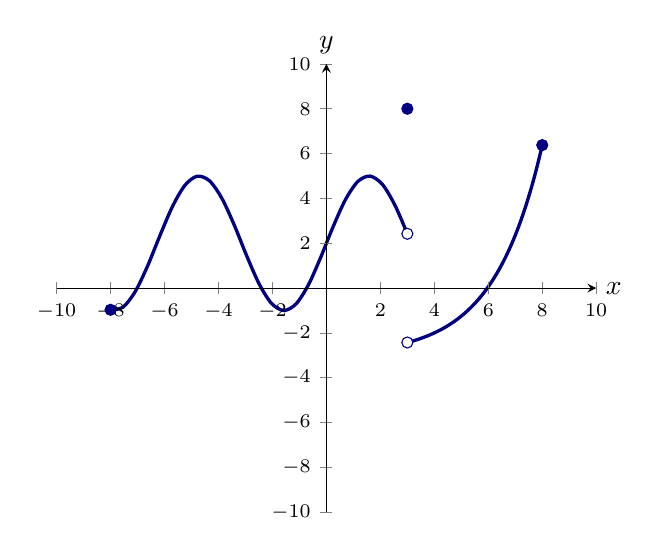
\begin{tikzpicture}
  \begin{axis}[
            domain=-10:10, ymax=10, xmax=10, ymin=-10, xmin=-10,
            axis lines =center, xlabel=$x$, ylabel=$y$,
            ytick={-10,-8,-6,-4,-2,2,4,6,8,10},
            xtick={-10,-8,-6,-4,-2,2,4,6,8,10},
            ticklabel style={font=\scriptsize},
            every axis y label/.style={at=(current axis.above origin),anchor=south},
            every axis x label/.style={at=(current axis.right of origin),anchor=west},
            axis on top
          ]
          
  \addplot [draw=penColor,very thick,smooth,domain=(-8:3)] {3*sin(deg(x)) + 2};
  \addplot [draw=penColor,very thick,smooth,domain=(3:8)] {(1.75^(x-4) - 3};
  \addplot[color=penColor,only marks,mark=*] coordinates{(-8,-0.968) (3,8) (8,6.378)}; 
  \addplot[color=penColor,fill=white,only marks,mark=*] coordinates{(3,2.423) (3,-2.428)}; 
  %\addplot[color=penColor,only marks,mark=*] coordinates{(1,2)}; 
  %\addplot[color=penColor,fill=white,only marks,mark=*] coordinates{(7,-4)}; 


    \end{axis}
\end{tikzpicture}
\end{image}




\begin{question}
The domain of $D$ is

\begin{multipleChoice}
  \choice {$(-8,3) \cup (3,8)$}
  \choice {$[-8,3) \cup (3,8]$}
  \choice [correct]{$[-8,8]$}
\end{multipleChoice}
\end{question}





\begin{question}
The range of $D$ is approximately

\begin{multipleChoice}
  \choice {$[0.97, 8]$}
  \choice {$(-2.43, 8]$}
  \choice {$(-2.43, 6.38) \cup \{ 8 \}$}
  \choice [correct]{$(-2.43, 6.38] \cup \{ 8 \}$}
\end{multipleChoice}
\end{question}



\begin{question}
The function $D$ has no minimum value
\begin{multipleChoice}
  \choice [correct]{True}
  \choice {False}
\end{multipleChoice}
\end{question}


\begin{question}
The function $D$ has no maximum value
\begin{multipleChoice}
  \choice {True}
  \choice [correct]{False}
\end{multipleChoice}
\end{question}




\end{example}




\begin{example}


The graph of a piecewise defined function may not look like pieces.



\[
f(x) = 
\begin{cases}
  \frac{1}{2} (x+8)^2 - \frac{21}{4} & \text{ if }  x \le -7 \\
  x + \frac{9}{4} & \text{ if }  -7 \leq x \leq \frac{5}{2} \\
  -(x-3)^2 + 5   & \text{ if } \frac{5}{2} \le v 
\end{cases}
\]






Graph of $y = f(x)$.
\begin{image}
\begin{tikzpicture}
  \begin{axis}[
            domain=-10:10, ymax=10, xmax=10, ymin=-10, xmin=-10,
            axis lines =center, xlabel=$x$, ylabel=$y$,
            ytick={-10,-8,-6,-4,-2,2,4,6,8,10},
            xtick={-10,-8,-6,-4,-2,2,4,6,8,10},
            ticklabel style={font=\scriptsize},
            every axis y label/.style={at=(current axis.above origin),anchor=south},
            every axis x label/.style={at=(current axis.right of origin),anchor=west},
            axis on top
          ]
          
        \addplot [draw=penColor,very thick,smooth,domain=(-9:-7),<-] {0.5*(x+8)^2 - 5.25};
        \addplot [draw=penColor,very thick,smooth,domain=(-7:2.5)] {x+2.25};
        \addplot [draw=penColor,very thick,smooth,domain=(2.5:6),->] {-(x-3)^2 + 5};



    \end{axis}
\end{tikzpicture}
\end{image}





\end{example}









\begin{center}
\textbf{\textcolor{green!50!black}{ooooo=-=-=-=-=-=-=-=-=-=-=-=-=ooOoo=-=-=-=-=-=-=-=-=-=-=-=-=ooooo}} \\

more examples can be found by following this link\\ \link[More Examples of Piecewise-Defined Functions]{https://ximera.osu.edu/csccmathematics/precalculus1/precalculus1/piecewise/examples/exampleList}

\end{center}









\end{document}
